%%%%%%%%%%%%%%%%%%%%%%%%%%%%%%%%%%%%%%%%%%%%%%%%%%%%%%%%%%%%%%%%%%%%%%
%%                     Not
%%%%%%%%%%%%%%%%%%%%%%%%%%%%%%%%%%%%%%%%%%%%%%%%%%%%%%%%%%%%%%%%%%%%%%
%\color{blue}
\subsection{Glyph: \glyph{Not}}\label{sec:not}

The glyph \glyph{not} is used to denote that the \glyph{EPN} linked as input cannot produce the output. \glyph{Not} is represented by a circle carrying the word ``NOT''.

\begin{figure}[H]
  \centering
  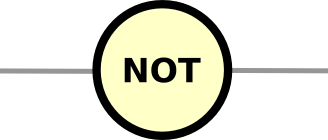
\includegraphics[scale = 0.5]{images/not}
  \caption{The \PD glyph for \glyph{not}.}
  \label{fig:not}
\end{figure}

